\section{Implementation}
\label{sec:impl}

Our approach to the DNS rebinding attack is derived from a standard time-varying attack, which can potentially take several minutes based on browser implementation of DNS Pinning. We discovered a previously undocumented variation which takes on the scale of tens of seconds. Instead of waiting for the pinned entries to expire, we flood the DNS cache with enough invalid entries to remove valid entries from the list. We plan to build on this idea and provide the attacker with a seamless browsing experience on the victim's internal server. We will retrieve the data from the victim's server (similar to existing scraping methods). Then we will allow the attacker to click links, take actions, and submit forms by sending the data to the victim's browser (which is acting as a proxy) and instruct it to send the appropriate request to the server.

We also plan to implement host discovery on the victim's internal network, so that no prior knowledge of the victim's network is required in order to execute the attack.

%use this:
Reference the figure like this: Figure \ref{fig:firedrill1}.

\begin{figure}[h]
\centering
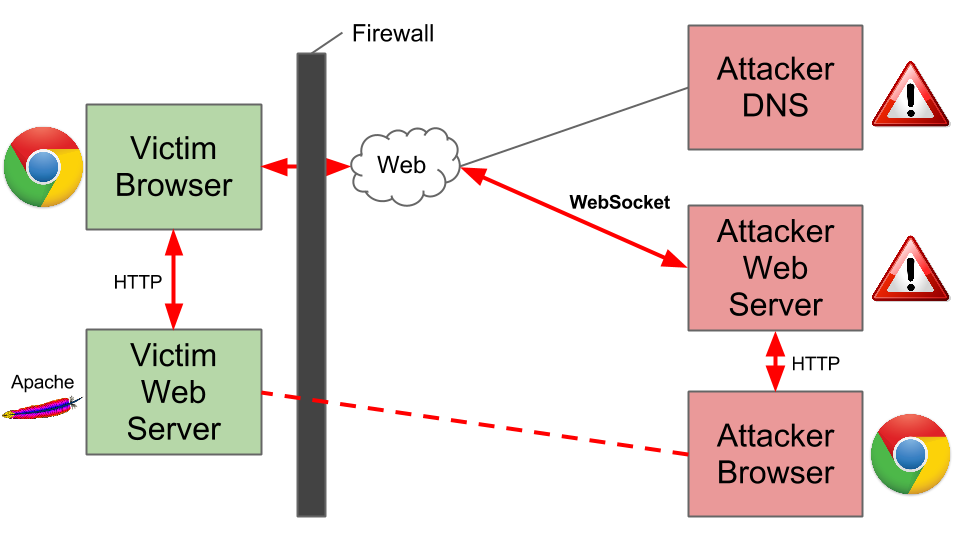
\includegraphics[width=0.8\columnwidth]{firedrill1.png}
\caption{\textbf{FireDrill Attack Overview.} Does xyz.}
\label{fig:firedrill1}
\end{figure}


